\documentclass[1p]{elsarticle_modified}
%\bibliographystyle{elsarticle-num}

%\usepackage[colorlinks]{hyperref}
%\usepackage{abbrmath_seonhwa} %\Abb, \Ascr, \Acal ,\Abf, \Afrak
\usepackage{amsfonts}
\usepackage{amssymb}
\usepackage{amsmath}
\usepackage{amsthm}
\usepackage{scalefnt}
\usepackage{amsbsy}
\usepackage{kotex}
\usepackage{caption}
\usepackage{subfig}
\usepackage{color}
\usepackage{graphicx}
\usepackage{xcolor} %% white, black, red, green, blue, cyan, magenta, yellow
\usepackage{float}
\usepackage{setspace}
\usepackage{hyperref}

\usepackage{tikz}
\usetikzlibrary{arrows}

\usepackage{multirow}
\usepackage{array} % fixed length table
\usepackage{hhline}

%%%%%%%%%%%%%%%%%%%%%
\makeatletter
\renewcommand*\env@matrix[1][\arraystretch]{%
	\edef\arraystretch{#1}%
	\hskip -\arraycolsep
	\let\@ifnextchar\new@ifnextchar
	\array{*\c@MaxMatrixCols c}}
\makeatother %https://tex.stackexchange.com/questions/14071/how-can-i-increase-the-line-spacing-in-a-matrix
%%%%%%%%%%%%%%%

\usepackage[normalem]{ulem}

\newcommand{\msout}[1]{\ifmmode\text{\sout{\ensuremath{#1}}}\else\sout{#1}\fi}
%SOURCE: \msout is \stkout macro in https://tex.stackexchange.com/questions/20609/strikeout-in-math-mode

\newcommand{\cancel}[1]{
	\ifmmode
	{\color{red}\msout{#1}}
	\else
	{\color{red}\sout{#1}}
	\fi
}

\newcommand{\add}[1]{
	{\color{blue}\uwave{#1}}
}

\newcommand{\replace}[2]{
	\ifmmode
	{\color{red}\msout{#1}}{\color{blue}\uwave{#2}}
	\else
	{\color{red}\sout{#1}}{\color{blue}\uwave{#2}}
	\fi
}

\newcommand{\Sol}{\mathcal{S}} %segment
\newcommand{\D}{D} %diagram
\newcommand{\A}{\mathcal{A}} %arc


%%%%%%%%%%%%%%%%%%%%%%%%%%%%%5 test

\def\sl{\operatorname{\textup{SL}}(2,\Cbb)}
\def\psl{\operatorname{\textup{PSL}}(2,\Cbb)}
\def\quan{\mkern 1mu \triangleright \mkern 1mu}

\theoremstyle{definition}
\newtheorem{thm}{Theorem}[section]
\newtheorem{prop}[thm]{Proposition}
\newtheorem{lem}[thm]{Lemma}
\newtheorem{ques}[thm]{Question}
\newtheorem{cor}[thm]{Corollary}
\newtheorem{defn}[thm]{Definition}
\newtheorem{exam}[thm]{Example}
\newtheorem{rmk}[thm]{Remark}
\newtheorem{alg}[thm]{Algorithm}

\newcommand{\I}{\sqrt{-1}}
\begin{document}

%\begin{frontmatter}
%
%\title{Boundary parabolic representations of knots up to 8 crossings}
%
%%% Group authors per affiliation:
%\author{Yunhi Cho} 
%\address{Department of Mathematics, University of Seoul, Seoul, Korea}
%\ead{yhcho@uos.ac.kr}
%
%
%\author{Seonhwa Kim} %\fnref{s_kim}}
%\address{Center for Geometry and Physics, Institute for Basic Science, Pohang, 37673, Korea}
%\ead{ryeona17@ibs.re.kr}
%
%\author{Hyuk Kim}
%\address{Department of Mathematical Sciences, Seoul National University, Seoul 08826, Korea}
%\ead{hyukkim@snu.ac.kr}
%
%\author{Seokbeom Yoon}
%\address{Department of Mathematical Sciences, Seoul National University, Seoul, 08826,  Korea}
%\ead{sbyoon15@snu.ac.kr}
%
%\begin{abstract}
%We find all boundary parabolic representation of knots up to 8 crossings.
%
%\end{abstract}
%\begin{keyword}
%    \MSC[2010] 57M25 
%\end{keyword}
%
%\end{frontmatter}

%\linenumbers
%\tableofcontents
%
\newcommand\colored[1]{\textcolor{white}{\rule[-0.35ex]{0.8em}{1.4ex}}\kern-0.8em\color{red} #1}%
%\newcommand\colored[1]{\textcolor{white}{ #1}\kern-2.17ex	\textcolor{white}{ #1}\kern-1.81ex	\textcolor{white}{ #1}\kern-2.15ex\color{red}#1	}

{\Large $\underline{12n_{0825}~(K12n_{0825})}$}

\setlength{\tabcolsep}{10pt}
\renewcommand{\arraystretch}{1.6}
\vspace{1cm}\begin{tabular}{m{100pt}>{\centering\arraybackslash}m{274pt}}
\multirow{5}{120pt}{
	\centering
	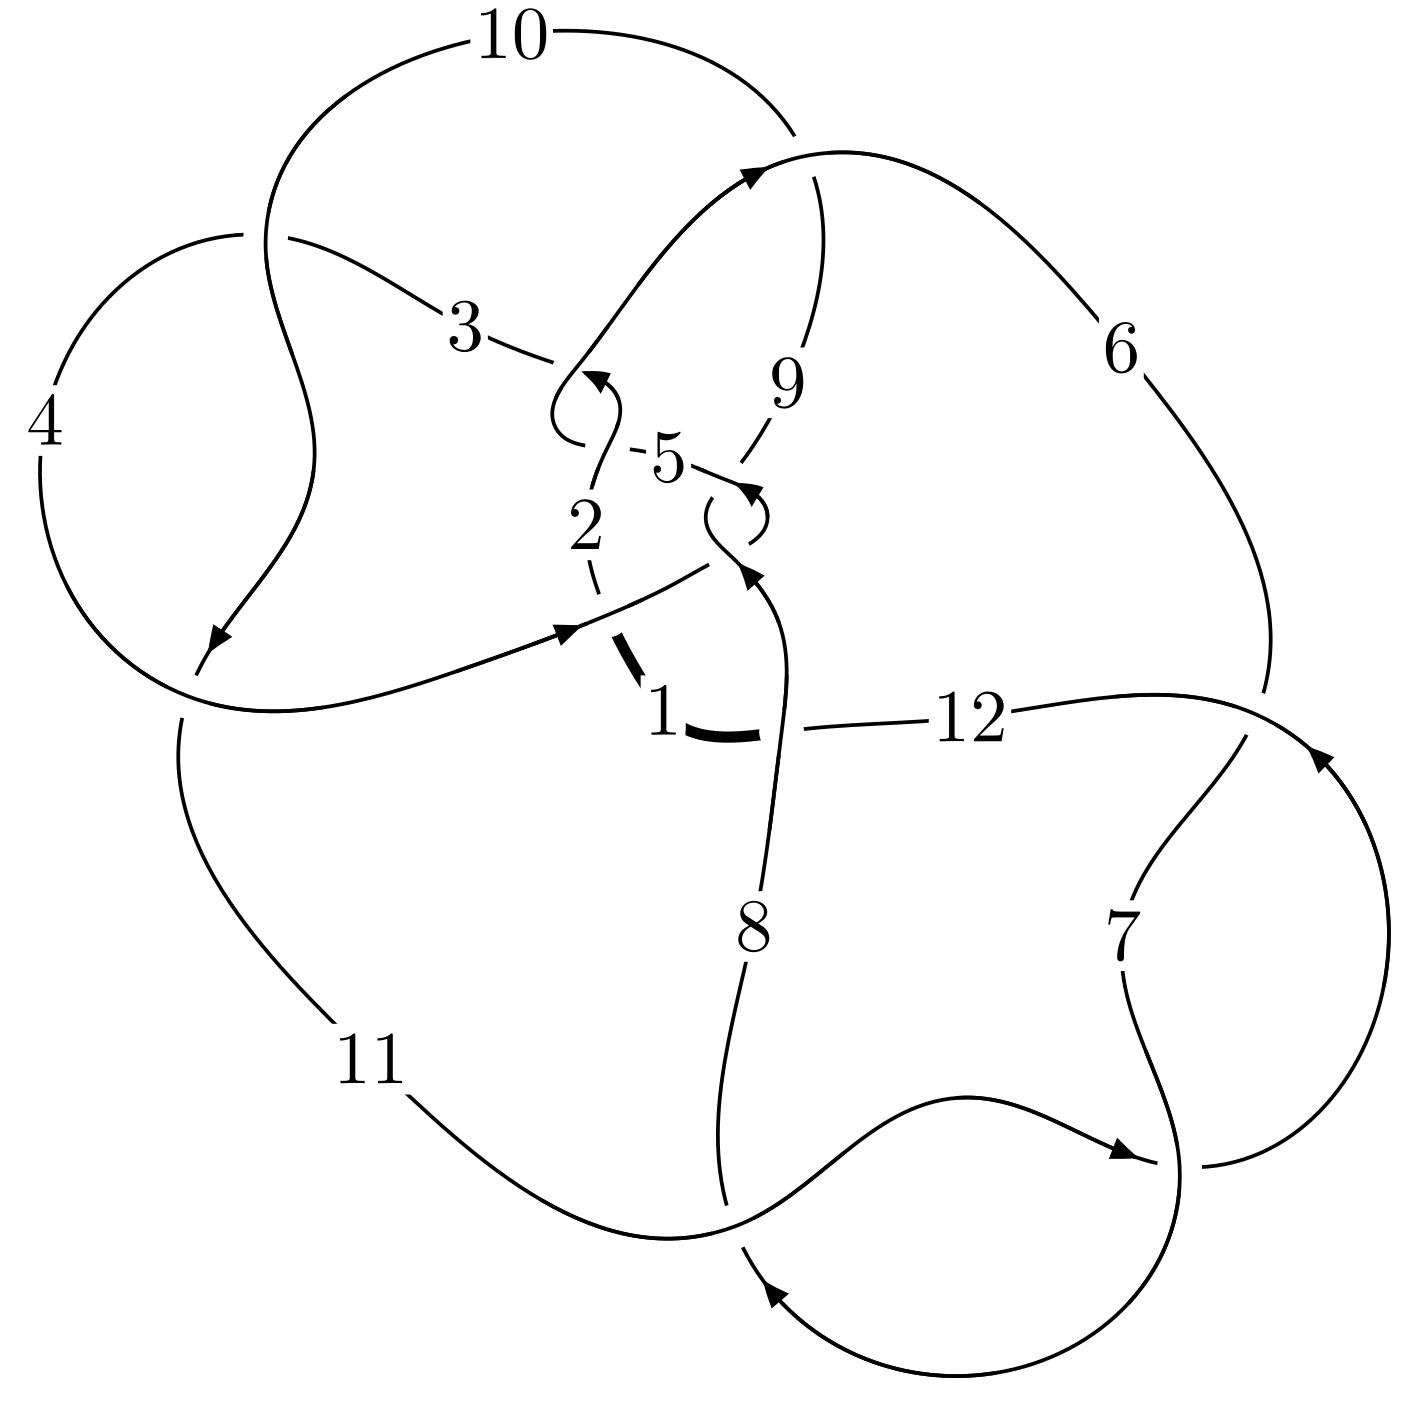
\includegraphics[width=112pt]{../../../GIT/diagram.site/Diagrams/png/2914_12n_0825.png}\\
\ \ \ A knot diagram\footnotemark}&
\allowdisplaybreaks
\textbf{Linearized knot diagam} \\
\cline{2-2}
 &
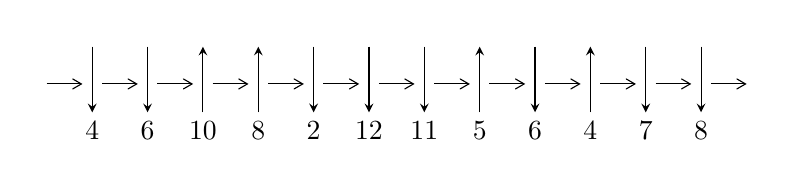
\begin{tikzpicture}[x=20pt, y=17pt]
	% nodes
	\node (C0) at (0, 0) {};
	\node (C1) at (1, 0) {};
	\node (C1U) at (1, +1) {};
	\node (C1D) at (1, -1) {4};

	\node (C2) at (2, 0) {};
	\node (C2U) at (2, +1) {};
	\node (C2D) at (2, -1) {6};

	\node (C3) at (3, 0) {};
	\node (C3U) at (3, +1) {};
	\node (C3D) at (3, -1) {10};

	\node (C4) at (4, 0) {};
	\node (C4U) at (4, +1) {};
	\node (C4D) at (4, -1) {8};

	\node (C5) at (5, 0) {};
	\node (C5U) at (5, +1) {};
	\node (C5D) at (5, -1) {2};

	\node (C6) at (6, 0) {};
	\node (C6U) at (6, +1) {};
	\node (C6D) at (6, -1) {12};

	\node (C7) at (7, 0) {};
	\node (C7U) at (7, +1) {};
	\node (C7D) at (7, -1) {11};

	\node (C8) at (8, 0) {};
	\node (C8U) at (8, +1) {};
	\node (C8D) at (8, -1) {5};

	\node (C9) at (9, 0) {};
	\node (C9U) at (9, +1) {};
	\node (C9D) at (9, -1) {6};

	\node (C10) at (10, 0) {};
	\node (C10U) at (10, +1) {};
	\node (C10D) at (10, -1) {4};

	\node (C11) at (11, 0) {};
	\node (C11U) at (11, +1) {};
	\node (C11D) at (11, -1) {7};

	\node (C12) at (12, 0) {};
	\node (C12U) at (12, +1) {};
	\node (C12D) at (12, -1) {8};
	\node (C13) at (13, 0) {};

	% arrows
	\draw[->,>={angle 60}]
	(C0) edge (C1) (C1) edge (C2) (C2) edge (C3) (C3) edge (C4) (C4) edge (C5) (C5) edge (C6) (C6) edge (C7) (C7) edge (C8) (C8) edge (C9) (C9) edge (C10) (C10) edge (C11) (C11) edge (C12) (C12) edge (C13) ;	\draw[->,>=stealth]
	(C1U) edge (C1D) (C2U) edge (C2D) (C3D) edge (C3U) (C4D) edge (C4U) (C5U) edge (C5D) (C6U) edge (C6D) (C7U) edge (C7D) (C8D) edge (C8U) (C9U) edge (C9D) (C10D) edge (C10U) (C11U) edge (C11D) (C12U) edge (C12D) ;
	\end{tikzpicture} \\
\hhline{~~} \\& 
\textbf{Solving Sequence} \\ \cline{2-2} 
 &
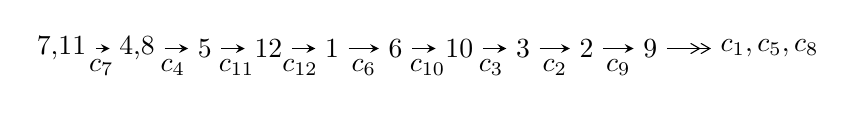
\begin{tikzpicture}[x=23pt, y=7pt]
	% node
	\node (A0) at (-1/8, 0) {7,11};
	\node (A1) at (17/16, 0) {4,8};
	\node (A2) at (17/8, 0) {5};
	\node (A3) at (25/8, 0) {12};
	\node (A4) at (33/8, 0) {1};
	\node (A5) at (41/8, 0) {6};
	\node (A6) at (49/8, 0) {10};
	\node (A7) at (57/8, 0) {3};
	\node (A8) at (65/8, 0) {2};
	\node (A9) at (73/8, 0) {9};
	\node (C1) at (1/2, -1) {$c_{7}$};
	\node (C2) at (13/8, -1) {$c_{4}$};
	\node (C3) at (21/8, -1) {$c_{11}$};
	\node (C4) at (29/8, -1) {$c_{12}$};
	\node (C5) at (37/8, -1) {$c_{6}$};
	\node (C6) at (45/8, -1) {$c_{10}$};
	\node (C7) at (53/8, -1) {$c_{3}$};
	\node (C8) at (61/8, -1) {$c_{2}$};
	\node (C9) at (69/8, -1) {$c_{9}$};
	\node (A10) at (11, 0) {$c_{1},c_{5},c_{8}$};

	% edge
	\draw[->,>=stealth]	
	(A0) edge (A1) (A1) edge (A2) (A2) edge (A3) (A3) edge (A4) (A4) edge (A5) (A5) edge (A6) (A6) edge (A7) (A7) edge (A8) (A8) edge (A9) ;
	\draw[->>,>={angle 60}]	
	(A9) edge (A10);
\end{tikzpicture} \\ 

\end{tabular} \\

\footnotetext{
The image of knot diagram is generated by the software ``\textbf{Draw programme}" developed by Andrew Bartholomew(\url{http://www.layer8.co.uk/maths/draw/index.htm\#Running-draw}), where we modified some parts for our purpose(\url{https://github.com/CATsTAILs/LinksPainter}).
}\phantom \\ \newline 
\centering \textbf{Ideals for irreducible components\footnotemark of $X_{\text{par}}$} 
 
\begin{align*}
I^u_{1}&=\langle 
- u^{17}+6 u^{16}+\cdots+2 b-2,\;- u^{17}+4 u^{16}+\cdots+4 a-8,\;u^{18}-6 u^{17}+\cdots+26 u-4\rangle \\
I^u_{2}&=\langle 
11 a^3 u^3-4 u^3 a^2+\cdots-5 a+29,\\
\phantom{I^u_{2}}&\phantom{= \langle  }a^3 u^3-5 u^3 a^2+a^4+2 a^3 u-2 a^2 u^2+6 u^3 a-12 a^2 u+5 u^2 a-10 u^3- a^2+15 a u-8 u^2+10 a-25 u-14,\\
\phantom{I^u_{2}}&\phantom{= \langle  }u^4+u^3+3 u^2+2 u+1\rangle \\
I^u_{3}&=\langle 
u^{11}+2 u^{10}+7 u^9+11 u^8+17 u^7+20 u^6+16 u^5+11 u^4+u^3-4 u^2+b-4 u-2,\\
\phantom{I^u_{3}}&\phantom{= \langle  }-2 u^{11}-2 u^{10}-13 u^9-11 u^8-30 u^7-21 u^6-26 u^5-14 u^4+2 u^3+u^2+a+10 u+2,\\
\phantom{I^u_{3}}&\phantom{= \langle  }u^{12}+u^{11}+7 u^{10}+6 u^9+18 u^8+13 u^7+19 u^6+11 u^5+3 u^4+u^3-6 u^2-2 u-1\rangle \\
\\
\end{align*}
\raggedright * 3 irreducible components of $\dim_{\mathbb{C}}=0$, with total 46 representations.\\
\footnotetext{All coefficients of polynomials are rational numbers. But the coefficients are sometimes approximated in decimal forms when there is not enough margin.}
\newpage
\renewcommand{\arraystretch}{1}
\centering \section*{I. $I^u_{1}= \langle - u^{17}+6 u^{16}+\cdots+2 b-2,\;- u^{17}+4 u^{16}+\cdots+4 a-8,\;u^{18}-6 u^{17}+\cdots+26 u-4 \rangle$}
\flushleft \textbf{(i) Arc colorings}\\
\begin{tabular}{m{7pt} m{180pt} m{7pt} m{180pt} }
\flushright $a_{7}=$&$\begin{pmatrix}1\\0\end{pmatrix}$ \\
\flushright $a_{11}=$&$\begin{pmatrix}0\\u\end{pmatrix}$ \\
\flushright $a_{4}=$&$\begin{pmatrix}\frac{1}{4} u^{17}- u^{16}+\cdots-\frac{45}{4} u+2\\\frac{1}{2} u^{17}-3 u^{16}+\cdots-\frac{15}{2} u+1\end{pmatrix}$ \\
\flushright $a_{8}=$&$\begin{pmatrix}1\\u^2\end{pmatrix}$ \\
\flushright $a_{5}=$&$\begin{pmatrix}-\frac{1}{4} u^{17}+u^{16}+\cdots-\frac{27}{4} u+1\\-\frac{1}{2} u^{17}+3 u^{16}+\cdots+\frac{33}{2} u-3\end{pmatrix}$ \\
\flushright $a_{12}=$&$\begin{pmatrix}- u\\u\end{pmatrix}$ \\
\flushright $a_{1}=$&$\begin{pmatrix}- u^3-2 u\\- u^5- u^3+u\end{pmatrix}$ \\
\flushright $a_{6}=$&$\begin{pmatrix}u^2+1\\- u^2\end{pmatrix}$ \\
\flushright $a_{10}=$&$\begin{pmatrix}- u^{17}+\frac{11}{2} u^{16}+\cdots+24 u-\frac{7}{2}\\\frac{1}{2} u^{17}-3 u^{16}+\cdots-\frac{25}{2} u+2\end{pmatrix}$ \\
\flushright $a_{3}=$&$\begin{pmatrix}\frac{1}{2} u^{17}-\frac{7}{2} u^{16}+\cdots-\frac{65}{2} u+\frac{13}{2}\\-\frac{1}{2} u^{17}+3 u^{16}+\cdots+\frac{19}{2} u-2\end{pmatrix}$ \\
\flushright $a_{2}=$&$\begin{pmatrix}-\frac{1}{2} u^{16}+2 u^{15}+\cdots-12 u+\frac{5}{2}\\-\frac{1}{2} u^{17}+3 u^{16}+\cdots+\frac{23}{2} u-2\end{pmatrix}$ \\
\flushright $a_{9}=$&$\begin{pmatrix}\frac{1}{2} u^{17}-\frac{5}{2} u^{16}+\cdots-\frac{3}{2} u+\frac{1}{2}\\-\frac{1}{2} u^{17}+3 u^{16}+\cdots+\frac{23}{2} u-2\end{pmatrix}$\\&\end{tabular}
\flushleft \textbf{(ii) Obstruction class $= -1$}\\~\\
\flushleft \textbf{(iii) Cusp Shapes $= - u^{17}+6 u^{16}-27 u^{15}+87 u^{14}-227 u^{13}+492 u^{12}-898 u^{11}+1405 u^{10}-1875 u^9+2132 u^8-2031 u^7+1572 u^6-916 u^5+322 u^4+39 u^3-138 u^2+90 u-26$}\\~\\
\newpage\renewcommand{\arraystretch}{1}
\flushleft \textbf{(iv) u-Polynomials at the component}\newline \\
\begin{tabular}{m{50pt}|m{274pt}}
Crossings & \hspace{64pt}u-Polynomials at each crossing \\
\hline $$\begin{aligned}c_{1}\end{aligned}$$&$\begin{aligned}
&u^{18}+3 u^{17}+\cdots+12 u-1
\end{aligned}$\\
\hline $$\begin{aligned}c_{2},c_{5}\end{aligned}$$&$\begin{aligned}
&u^{18}+12 u^{17}+\cdots-96 u-16
\end{aligned}$\\
\hline $$\begin{aligned}c_{3},c_{4},c_{8}\\c_{10}\end{aligned}$$&$\begin{aligned}
&u^{18}- u^{17}+\cdots- u+1
\end{aligned}$\\
\hline $$\begin{aligned}c_{6},c_{7},c_{11}\end{aligned}$$&$\begin{aligned}
&u^{18}+6 u^{17}+\cdots-26 u-4
\end{aligned}$\\
\hline $$\begin{aligned}c_{9}\end{aligned}$$&$\begin{aligned}
&u^{18}- u^{17}+\cdots+11 u-1
\end{aligned}$\\
\hline $$\begin{aligned}c_{12}\end{aligned}$$&$\begin{aligned}
&u^{18}-6 u^{17}+\cdots-584 u-712
\end{aligned}$\\
\hline
\end{tabular}\\~\\
\newpage\renewcommand{\arraystretch}{1}
\flushleft \textbf{(v) Riley Polynomials at the component}\newline \\
\begin{tabular}{m{50pt}|m{274pt}}
Crossings & \hspace{64pt}Riley Polynomials at each crossing \\
\hline $$\begin{aligned}c_{1}\end{aligned}$$&$\begin{aligned}
&y^{18}+37 y^{17}+\cdots-62 y+1
\end{aligned}$\\
\hline $$\begin{aligned}c_{2},c_{5}\end{aligned}$$&$\begin{aligned}
&y^{18}-4 y^{17}+\cdots-640 y+256
\end{aligned}$\\
\hline $$\begin{aligned}c_{3},c_{4},c_{8}\\c_{10}\end{aligned}$$&$\begin{aligned}
&y^{18}-25 y^{17}+\cdots-9 y+1
\end{aligned}$\\
\hline $$\begin{aligned}c_{6},c_{7},c_{11}\end{aligned}$$&$\begin{aligned}
&y^{18}+18 y^{17}+\cdots-28 y+16
\end{aligned}$\\
\hline $$\begin{aligned}c_{9}\end{aligned}$$&$\begin{aligned}
&y^{18}+33 y^{17}+\cdots-83 y+1
\end{aligned}$\\
\hline $$\begin{aligned}c_{12}\end{aligned}$$&$\begin{aligned}
&y^{18}+10 y^{17}+\cdots+1367744 y+506944
\end{aligned}$\\
\hline
\end{tabular}\\~\\
\newpage\flushleft \textbf{(vi) Complex Volumes and Cusp Shapes}
$$\begin{array}{c|c|c}  
\text{Solutions to }I^u_{1}& \I (\text{vol} + \sqrt{-1}CS) & \text{Cusp shape}\\
 \hline 
\begin{aligned}
u &= \phantom{-}0.916911 + 0.561321 I \\
a &= \phantom{-}1.37834 - 0.77557 I \\
b &= -0.176299 + 0.948574 I\end{aligned}
 & \phantom{-}13.57260 + 1.61994 I & \phantom{-}0.247785 + 0.097983 I \\ \hline\begin{aligned}
u &= \phantom{-}0.916911 - 0.561321 I \\
a &= \phantom{-}1.37834 + 0.77557 I \\
b &= -0.176299 - 0.948574 I\end{aligned}
 & \phantom{-}13.57260 - 1.61994 I & \phantom{-}0.247785 - 0.097983 I \\ \hline\begin{aligned}
u &= \phantom{-}0.874769 + 0.633678 I \\
a &= -1.17600 + 1.10821 I \\
b &= \phantom{-}0.074687 - 1.124960 I\end{aligned}
 & \phantom{-}13.8091 - 7.5293 I & \phantom{-}0.29015 + 4.49288 I \\ \hline\begin{aligned}
u &= \phantom{-}0.874769 - 0.633678 I \\
a &= -1.17600 - 1.10821 I \\
b &= \phantom{-}0.074687 + 1.124960 I\end{aligned}
 & \phantom{-}13.8091 + 7.5293 I & \phantom{-}0.29015 - 4.49288 I \\ \hline\begin{aligned}
u &= \phantom{-}0.733837\phantom{ +0.000000I} \\
a &= -0.784391\phantom{ +0.000000I} \\
b &= \phantom{-}0.153207\phantom{ +0.000000I}\end{aligned}
 & -2.09100\phantom{ +0.000000I} & -1.44720\phantom{ +0.000000I} \\ \hline\begin{aligned}
u &= \phantom{-}0.310769 + 1.286500 I \\
a &= \phantom{-}0.184515 - 0.432647 I \\
b &= -0.555563 + 0.718899 I\end{aligned}
 & \phantom{-}1.93032 - 3.76798 I & \phantom{-}2.83080 + 5.29800 I \\ \hline\begin{aligned}
u &= \phantom{-}0.310769 - 1.286500 I \\
a &= \phantom{-}0.184515 + 0.432647 I \\
b &= -0.555563 - 0.718899 I\end{aligned}
 & \phantom{-}1.93032 + 3.76798 I & \phantom{-}2.83080 - 5.29800 I \\ \hline\begin{aligned}
u &= \phantom{-}0.054735 + 1.390450 I \\
a &= \phantom{-}0.429200 + 0.371775 I \\
b &= -0.391654 - 1.269460 I\end{aligned}
 & \phantom{-}5.15709 - 2.04112 I & \phantom{-}0.57723 + 3.95110 I \\ \hline\begin{aligned}
u &= \phantom{-}0.054735 - 1.390450 I \\
a &= \phantom{-}0.429200 - 0.371775 I \\
b &= -0.391654 + 1.269460 I\end{aligned}
 & \phantom{-}5.15709 + 2.04112 I & \phantom{-}0.57723 - 3.95110 I \\ \hline\begin{aligned}
u &= -0.186935 + 1.380880 I \\
a &= -0.380579 - 0.441876 I \\
b &= -0.19705 + 1.46656 I\end{aligned}
 & \phantom{-}1.96657 + 2.47572 I & \phantom{-}0.511687 + 1.171098 I\\
 \hline 
 \end{array}$$\newpage$$\begin{array}{c|c|c}  
\text{Solutions to }I^u_{1}& \I (\text{vol} + \sqrt{-1}CS) & \text{Cusp shape}\\
 \hline 
\begin{aligned}
u &= -0.186935 - 1.380880 I \\
a &= -0.380579 + 0.441876 I \\
b &= -0.19705 - 1.46656 I\end{aligned}
 & \phantom{-}1.96657 - 2.47572 I & \phantom{-}0.511687 - 1.171098 I \\ \hline\begin{aligned}
u &= -0.510799\phantom{ +0.000000I} \\
a &= \phantom{-}0.933996\phantom{ +0.000000I} \\
b &= \phantom{-}0.720779\phantom{ +0.000000I}\end{aligned}
 & -2.51252\phantom{ +0.000000I} & \phantom{-}3.72050\phantom{ +0.000000I} \\ \hline\begin{aligned}
u &= \phantom{-}0.280643 + 0.301264 I \\
a &= -0.588140 - 1.071850 I \\
b &= \phantom{-}0.030449 + 0.391403 I\end{aligned}
 & -0.225777 - 0.895913 I & -4.68203 + 7.75983 I \\ \hline\begin{aligned}
u &= \phantom{-}0.280643 - 0.301264 I \\
a &= -0.588140 + 1.071850 I \\
b &= \phantom{-}0.030449 - 0.391403 I\end{aligned}
 & -0.225777 + 0.895913 I & -4.68203 - 7.75983 I \\ \hline\begin{aligned}
u &= \phantom{-}0.33904 + 1.59351 I \\
a &= -0.148834 + 1.046660 I \\
b &= \phantom{-}0.94820 - 2.81595 I\end{aligned}
 & -18.8931 - 3.0610 I & \phantom{-}2.60805 + 0.97919 I \\ \hline\begin{aligned}
u &= \phantom{-}0.33904 - 1.59351 I \\
a &= -0.148834 - 1.046660 I \\
b &= \phantom{-}0.94820 + 2.81595 I\end{aligned}
 & -18.8931 + 3.0610 I & \phantom{-}2.60805 - 0.97919 I \\ \hline\begin{aligned}
u &= \phantom{-}0.29855 + 1.60658 I \\
a &= -0.023307 - 1.135190 I \\
b &= -0.66976 + 3.18283 I\end{aligned}
 & -18.3049 - 11.9078 I & \phantom{-}2.47969 + 4.91668 I \\ \hline\begin{aligned}
u &= \phantom{-}0.29855 - 1.60658 I \\
a &= -0.023307 + 1.135190 I \\
b &= -0.66976 - 3.18283 I\end{aligned}
 & -18.3049 + 11.9078 I & \phantom{-}2.47969 - 4.91668 I\\
 \hline 
 \end{array}$$\newpage\newpage\renewcommand{\arraystretch}{1}
\centering \section*{II. $I^u_{2}= \langle 11 a^3 u^3-4 u^3 a^2+\cdots-5 a+29,\;a^3 u^3-5 u^3 a^2+\cdots+10 a-14,\;u^4+u^3+3 u^2+2 u+1 \rangle$}
\flushleft \textbf{(i) Arc colorings}\\
\begin{tabular}{m{7pt} m{180pt} m{7pt} m{180pt} }
\flushright $a_{7}=$&$\begin{pmatrix}1\\0\end{pmatrix}$ \\
\flushright $a_{11}=$&$\begin{pmatrix}0\\u\end{pmatrix}$ \\
\flushright $a_{4}=$&$\begin{pmatrix}a\\-0.354839 a^{3} u^{3}+0.129032 a^{2} u^{3}+\cdots+0.161290 a-0.935484\end{pmatrix}$ \\
\flushright $a_{8}=$&$\begin{pmatrix}1\\u^2\end{pmatrix}$ \\
\flushright $a_{5}=$&$\begin{pmatrix}-0.354839 a^{3} u^{3}+0.129032 a^{2} u^{3}+\cdots+1.16129 a-0.935484\\0.677419 a^{3} u^{3}-0.0645161 a^{2} u^{3}+\cdots+0.419355 a-0.0322581\end{pmatrix}$ \\
\flushright $a_{12}=$&$\begin{pmatrix}- u\\u\end{pmatrix}$ \\
\flushright $a_{1}=$&$\begin{pmatrix}- u^3-2 u\\u^3- u^2-1\end{pmatrix}$ \\
\flushright $a_{6}=$&$\begin{pmatrix}u^2+1\\- u^2\end{pmatrix}$ \\
\flushright $a_{10}=$&$\begin{pmatrix}- a^2 u\\0.193548 a^{3} u^{3}-1.16129 a^{2} u^{3}+\cdots+0.548387 a-0.580645\end{pmatrix}$ \\
\flushright $a_{3}=$&$\begin{pmatrix}- a^3 u^2+a\\0.387097 a^{3} u^{3}-0.322581 a^{2} u^{3}+\cdots+0.0967742 a-1.16129\end{pmatrix}$ \\
\flushright $a_{2}=$&$\begin{pmatrix}0.0967742 a^{3} u^{3}-0.580645 a^{2} u^{3}+\cdots+0.774194 a-1.29032\\0.0967742 a^{3} u^{3}+0.419355 a^{2} u^{3}+\cdots-0.225806 a-1.29032\end{pmatrix}$ \\
\flushright $a_{9}=$&$\begin{pmatrix}0.548387 a^{3} u^{3}-0.290323 a^{2} u^{3}+\cdots+0.387097 a+1.35484\\-0.451613 a^{3} u^{3}-0.290323 a^{2} u^{3}+\cdots+0.387097 a-2.64516\end{pmatrix}$\\&\end{tabular}
\flushleft \textbf{(ii) Obstruction class $= -1$}\\~\\
\flushleft \textbf{(iii) Cusp Shapes $= \frac{24}{31} a^3 u^3+\frac{84}{31} a^3 u^2-\frac{20}{31} u^3 a^2+\frac{96}{31} a^3 u-\frac{8}{31} a^2 u^2+\frac{16}{31} u^3 a+\frac{40}{31} a^3+\frac{44}{31} a^2 u+\frac{56}{31} u^2 a-\frac{68}{31} u^3+\frac{8}{31} a^2+\frac{64}{31} a u-\frac{52}{31} u^2+\frac{68}{31} a-\frac{148}{31} u-\frac{10}{31}$}\\~\\
\newpage\renewcommand{\arraystretch}{1}
\flushleft \textbf{(iv) u-Polynomials at the component}\newline \\
\begin{tabular}{m{50pt}|m{274pt}}
Crossings & \hspace{64pt}u-Polynomials at each crossing \\
\hline $$\begin{aligned}c_{1}\end{aligned}$$&$\begin{aligned}
&u^{16}-7 u^{15}+\cdots-478 u+73
\end{aligned}$\\
\hline $$\begin{aligned}c_{2},c_{5}\end{aligned}$$&$\begin{aligned}
&(u^2- u+1)^8
\end{aligned}$\\
\hline $$\begin{aligned}c_{3},c_{4},c_{8}\\c_{10}\end{aligned}$$&$\begin{aligned}
&u^{16}+u^{15}+\cdots-24 u+79
\end{aligned}$\\
\hline $$\begin{aligned}c_{6},c_{7},c_{11}\end{aligned}$$&$\begin{aligned}
&(u^4- u^3+3 u^2-2 u+1)^4
\end{aligned}$\\
\hline $$\begin{aligned}c_{9}\end{aligned}$$&$\begin{aligned}
&u^{16}+3 u^{15}+\cdots+180 u+79
\end{aligned}$\\
\hline $$\begin{aligned}c_{12}\end{aligned}$$&$\begin{aligned}
&(u^4+u^3+5 u^2- u+2)^4
\end{aligned}$\\
\hline
\end{tabular}\\~\\
\newpage\renewcommand{\arraystretch}{1}
\flushleft \textbf{(v) Riley Polynomials at the component}\newline \\
\begin{tabular}{m{50pt}|m{274pt}}
Crossings & \hspace{64pt}Riley Polynomials at each crossing \\
\hline $$\begin{aligned}c_{1}\end{aligned}$$&$\begin{aligned}
&y^{16}+27 y^{15}+\cdots+40448 y+5329
\end{aligned}$\\
\hline $$\begin{aligned}c_{2},c_{5}\end{aligned}$$&$\begin{aligned}
&(y^2+y+1)^8
\end{aligned}$\\
\hline $$\begin{aligned}c_{3},c_{4},c_{8}\\c_{10}\end{aligned}$$&$\begin{aligned}
&y^{16}-21 y^{15}+\cdots-51768 y+6241
\end{aligned}$\\
\hline $$\begin{aligned}c_{6},c_{7},c_{11}\end{aligned}$$&$\begin{aligned}
&(y^4+5 y^3+7 y^2+2 y+1)^4
\end{aligned}$\\
\hline $$\begin{aligned}c_{9}\end{aligned}$$&$\begin{aligned}
&y^{16}+23 y^{15}+\cdots+58924 y+6241
\end{aligned}$\\
\hline $$\begin{aligned}c_{12}\end{aligned}$$&$\begin{aligned}
&(y^4+9 y^3+31 y^2+19 y+4)^4
\end{aligned}$\\
\hline
\end{tabular}\\~\\
\newpage\flushleft \textbf{(vi) Complex Volumes and Cusp Shapes}
$$\begin{array}{c|c|c}  
\text{Solutions to }I^u_{2}& \I (\text{vol} + \sqrt{-1}CS) & \text{Cusp shape}\\
 \hline 
\begin{aligned}
u &= -0.395123 + 0.506844 I \\
a &= \phantom{-}0.918767 + 0.732292 I \\
b &= -1.333200 - 0.320958 I\end{aligned}
 & \phantom{-}4.72380 - 0.61478 I & \phantom{-}0.17326 - 1.44464 I \\ \hline\begin{aligned}
u &= -0.395123 + 0.506844 I \\
a &= \phantom{-}0.17223 - 1.96502 I \\
b &= \phantom{-}0.571429 + 0.327901 I\end{aligned}
 & \phantom{-}4.72380 + 3.44499 I & \phantom{-}0.17326 - 8.37284 I \\ \hline\begin{aligned}
u &= -0.395123 + 0.506844 I \\
a &= \phantom{-}1.07219 + 1.87866 I \\
b &= -0.28348 - 1.48247 I\end{aligned}
 & \phantom{-}4.72380 + 3.44499 I & \phantom{-}0.17326 - 8.37284 I \\ \hline\begin{aligned}
u &= -0.395123 + 0.506844 I \\
a &= -1.61576 - 1.76681 I \\
b &= \phantom{-}0.189337 + 0.648876 I\end{aligned}
 & \phantom{-}4.72380 - 0.61478 I & \phantom{-}0.17326 - 1.44464 I \\ \hline\begin{aligned}
u &= -0.395123 - 0.506844 I \\
a &= \phantom{-}0.918767 - 0.732292 I \\
b &= -1.333200 + 0.320958 I\end{aligned}
 & \phantom{-}4.72380 + 0.61478 I & \phantom{-}0.17326 + 1.44464 I \\ \hline\begin{aligned}
u &= -0.395123 - 0.506844 I \\
a &= \phantom{-}0.17223 + 1.96502 I \\
b &= \phantom{-}0.571429 - 0.327901 I\end{aligned}
 & \phantom{-}4.72380 - 3.44499 I & \phantom{-}0.17326 + 8.37284 I \\ \hline\begin{aligned}
u &= -0.395123 - 0.506844 I \\
a &= \phantom{-}1.07219 - 1.87866 I \\
b &= -0.28348 + 1.48247 I\end{aligned}
 & \phantom{-}4.72380 - 3.44499 I & \phantom{-}0.17326 + 8.37284 I \\ \hline\begin{aligned}
u &= -0.395123 - 0.506844 I \\
a &= -1.61576 + 1.76681 I \\
b &= \phantom{-}0.189337 - 0.648876 I\end{aligned}
 & \phantom{-}4.72380 + 0.61478 I & \phantom{-}0.17326 + 1.44464 I \\ \hline\begin{aligned}
u &= -0.10488 + 1.55249 I \\
a &= \phantom{-}0.084078 - 0.977337 I \\
b &= \phantom{-}0.62521 + 3.74384 I\end{aligned}
 & \phantom{-}11.72550 + 5.19385 I & \phantom{-}3.82674 - 6.02890 I \\ \hline\begin{aligned}
u &= -0.10488 + 1.55249 I \\
a &= -0.864979 + 0.796080 I \\
b &= \phantom{-}0.82603 - 1.86134 I\end{aligned}
 & \phantom{-}11.72550 + 5.19385 I & \phantom{-}3.82674 - 6.02890 I\\
 \hline 
 \end{array}$$\newpage$$\begin{array}{c|c|c}  
\text{Solutions to }I^u_{2}& \I (\text{vol} + \sqrt{-1}CS) & \text{Cusp shape}\\
 \hline 
\begin{aligned}
u &= -0.10488 + 1.55249 I \\
a &= \phantom{-}0.050829 + 1.247660 I \\
b &= -0.44287 - 3.34396 I\end{aligned}
 & \phantom{-}11.72550 + 1.13408 I & \phantom{-}3.82674 + 0.89930 I \\ \hline\begin{aligned}
u &= -0.10488 + 1.55249 I \\
a &= \phantom{-}0.182649 - 0.480753 I \\
b &= \phantom{-}1.34755 + 1.14590 I\end{aligned}
 & \phantom{-}11.72550 + 1.13408 I & \phantom{-}3.82674 + 0.89930 I \\ \hline\begin{aligned}
u &= -0.10488 - 1.55249 I \\
a &= \phantom{-}0.084078 + 0.977337 I \\
b &= \phantom{-}0.62521 - 3.74384 I\end{aligned}
 & \phantom{-}11.72550 - 5.19385 I & \phantom{-}3.82674 + 6.02890 I \\ \hline\begin{aligned}
u &= -0.10488 - 1.55249 I \\
a &= -0.864979 - 0.796080 I \\
b &= \phantom{-}0.82603 + 1.86134 I\end{aligned}
 & \phantom{-}11.72550 - 5.19385 I & \phantom{-}3.82674 + 6.02890 I \\ \hline\begin{aligned}
u &= -0.10488 - 1.55249 I \\
a &= \phantom{-}0.050829 - 1.247660 I \\
b &= -0.44287 + 3.34396 I\end{aligned}
 & \phantom{-}11.72550 - 1.13408 I & \phantom{-}3.82674 - 0.89930 I \\ \hline\begin{aligned}
u &= -0.10488 - 1.55249 I \\
a &= \phantom{-}0.182649 + 0.480753 I \\
b &= \phantom{-}1.34755 - 1.14590 I\end{aligned}
 & \phantom{-}11.72550 - 1.13408 I & \phantom{-}3.82674 - 0.89930 I\\
 \hline 
 \end{array}$$\newpage\newpage\renewcommand{\arraystretch}{1}
\centering \section*{III. $I^u_{3}= \langle u^{11}+2 u^{10}+\cdots+b-2,\;-2 u^{11}-2 u^{10}+\cdots+a+2,\;u^{12}+u^{11}+\cdots-2 u-1 \rangle$}
\flushleft \textbf{(i) Arc colorings}\\
\begin{tabular}{m{7pt} m{180pt} m{7pt} m{180pt} }
\flushright $a_{7}=$&$\begin{pmatrix}1\\0\end{pmatrix}$ \\
\flushright $a_{11}=$&$\begin{pmatrix}0\\u\end{pmatrix}$ \\
\flushright $a_{4}=$&$\begin{pmatrix}2 u^{11}+2 u^{10}+\cdots-10 u-2\\- u^{11}-2 u^{10}+\cdots+4 u+2\end{pmatrix}$ \\
\flushright $a_{8}=$&$\begin{pmatrix}1\\u^2\end{pmatrix}$ \\
\flushright $a_{5}=$&$\begin{pmatrix}2 u^{11}+u^{10}+12 u^9+5 u^8+25 u^7+9 u^6+18 u^5+6 u^4-5 u^3+u^2-8 u\\- u^{11}- u^{10}-6 u^9-5 u^8-12 u^7-9 u^6-8 u^5-6 u^4+2 u^3+2 u+1\end{pmatrix}$ \\
\flushright $a_{12}=$&$\begin{pmatrix}- u\\u\end{pmatrix}$ \\
\flushright $a_{1}=$&$\begin{pmatrix}- u^3-2 u\\- u^5- u^3+u\end{pmatrix}$ \\
\flushright $a_{6}=$&$\begin{pmatrix}u^2+1\\- u^2\end{pmatrix}$ \\
\flushright $a_{10}=$&$\begin{pmatrix}-2 u^{11}- u^{10}+\cdots+12 u+1\\u^{11}+5 u^9+9 u^7+u^6+6 u^5+3 u^4- u^3+3 u^2-2 u-1\end{pmatrix}$ \\
\flushright $a_{3}=$&$\begin{pmatrix}- u^{11}- u^{10}+\cdots+7 u-2\\- u^{11}-4 u^9+u^8-3 u^7+4 u^6+5 u^5+4 u^4+5 u^3- u^2-3 u-1\end{pmatrix}$ \\
\flushright $a_{2}=$&$\begin{pmatrix}- u^{11}- u^{10}-7 u^9-5 u^8-17 u^7-8 u^6-15 u^5-3 u^4+u^3+u^2+5 u-2\\u^{10}+2 u^9+6 u^8+9 u^7+12 u^6+12 u^5+7 u^4+2 u^3-3 u^2-4 u-1\end{pmatrix}$ \\
\flushright $a_{9}=$&$\begin{pmatrix}- u^{11}-7 u^9- u^8-18 u^7-4 u^6-18 u^5-5 u^4-2 u^2+9 u\\- u^{10}-4 u^8+u^7-4 u^6+3 u^5+2 u^4+2 u^3+4 u^2-2 u-1\end{pmatrix}$\\&\end{tabular}
\flushleft \textbf{(ii) Obstruction class $= 1$}\\~\\
\flushleft \textbf{(iii) Cusp Shapes $= 2 u^{11}+3 u^{10}+13 u^9+15 u^8+28 u^7+20 u^6+16 u^5-5 u^4-15 u^3-19 u^2-13 u+1$}\\~\\
\newpage\renewcommand{\arraystretch}{1}
\flushleft \textbf{(iv) u-Polynomials at the component}\newline \\
\begin{tabular}{m{50pt}|m{274pt}}
Crossings & \hspace{64pt}u-Polynomials at each crossing \\
\hline $$\begin{aligned}c_{1}\end{aligned}$$&$\begin{aligned}
&u^{12}+3 u^{11}+\cdots-3 u-1
\end{aligned}$\\
\hline $$\begin{aligned}c_{2}\end{aligned}$$&$\begin{aligned}
&u^{12}+3 u^{11}+\cdots-3 u-1
\end{aligned}$\\
\hline $$\begin{aligned}c_{3},c_{8}\end{aligned}$$&$\begin{aligned}
&u^{12}+u^{11}+\cdots-10 u^2+1
\end{aligned}$\\
\hline $$\begin{aligned}c_{4},c_{10}\end{aligned}$$&$\begin{aligned}
&u^{12}- u^{11}+\cdots-10 u^2+1
\end{aligned}$\\
\hline $$\begin{aligned}c_{5}\end{aligned}$$&$\begin{aligned}
&u^{12}-3 u^{11}+\cdots+3 u-1
\end{aligned}$\\
\hline $$\begin{aligned}c_{6},c_{7}\end{aligned}$$&$\begin{aligned}
&u^{12}+u^{11}+\cdots-2 u-1
\end{aligned}$\\
\hline $$\begin{aligned}c_{9}\end{aligned}$$&$\begin{aligned}
&u^{12}+u^{11}+4 u^{10}+2 u^9+6 u^8+u^7+6 u^6- u^5+u^4+4 u^3+3 u^2-1
\end{aligned}$\\
\hline $$\begin{aligned}c_{11}\end{aligned}$$&$\begin{aligned}
&u^{12}- u^{11}+\cdots+2 u-1
\end{aligned}$\\
\hline $$\begin{aligned}c_{12}\end{aligned}$$&$\begin{aligned}
&u^{12}+u^{11}+u^{10}-3 u^9-11 u^8+8 u^7+18 u^6-9 u^5-12 u^4-9 u^3-7 u^2-1
\end{aligned}$\\
\hline
\end{tabular}\\~\\
\newpage\renewcommand{\arraystretch}{1}
\flushleft \textbf{(v) Riley Polynomials at the component}\newline \\
\begin{tabular}{m{50pt}|m{274pt}}
Crossings & \hspace{64pt}Riley Polynomials at each crossing \\
\hline $$\begin{aligned}c_{1}\end{aligned}$$&$\begin{aligned}
&y^{12}+3 y^{11}+\cdots-5 y+1
\end{aligned}$\\
\hline $$\begin{aligned}c_{2},c_{5}\end{aligned}$$&$\begin{aligned}
&y^{12}-5 y^{11}+\cdots+3 y+1
\end{aligned}$\\
\hline $$\begin{aligned}c_{3},c_{4},c_{8}\\c_{10}\end{aligned}$$&$\begin{aligned}
&y^{12}-15 y^{11}+\cdots-20 y+1
\end{aligned}$\\
\hline $$\begin{aligned}c_{6},c_{7},c_{11}\end{aligned}$$&$\begin{aligned}
&y^{12}+13 y^{11}+\cdots+8 y+1
\end{aligned}$\\
\hline $$\begin{aligned}c_{9}\end{aligned}$$&$\begin{aligned}
&y^{12}+7 y^{11}+\cdots-6 y+1
\end{aligned}$\\
\hline $$\begin{aligned}c_{12}\end{aligned}$$&$\begin{aligned}
&y^{12}+y^{11}+\cdots+14 y+1
\end{aligned}$\\
\hline
\end{tabular}\\~\\
\newpage\flushleft \textbf{(vi) Complex Volumes and Cusp Shapes}
$$\begin{array}{c|c|c}  
\text{Solutions to }I^u_{3}& \I (\text{vol} + \sqrt{-1}CS) & \text{Cusp shape}\\
 \hline 
\begin{aligned}
u &= -0.840044\phantom{ +0.000000I} \\
a &= \phantom{-}1.57497\phantom{ +0.000000I} \\
b &= -0.211629\phantom{ +0.000000I}\end{aligned}
 & \phantom{-}0.654628\phantom{ +0.000000I} & -1.77310\phantom{ +0.000000I} \\ \hline\begin{aligned}
u &= -0.042760 + 1.221860 I \\
a &= \phantom{-}0.288630 + 0.954256 I \\
b &= -1.50897 - 1.14119 I\end{aligned}
 & \phantom{-}7.97414 - 1.59154 I & \phantom{-}3.95302 + 1.55241 I \\ \hline\begin{aligned}
u &= -0.042760 - 1.221860 I \\
a &= \phantom{-}0.288630 - 0.954256 I \\
b &= -1.50897 + 1.14119 I\end{aligned}
 & \phantom{-}7.97414 + 1.59154 I & \phantom{-}3.95302 - 1.55241 I \\ \hline\begin{aligned}
u &= -0.375195 + 1.251700 I \\
a &= -0.224979 - 0.971377 I \\
b &= \phantom{-}0.70872 + 1.67932 I\end{aligned}
 & \phantom{-}4.52363 + 4.37134 I & \phantom{-}1.55173 - 4.04786 I \\ \hline\begin{aligned}
u &= -0.375195 - 1.251700 I \\
a &= -0.224979 + 0.971377 I \\
b &= \phantom{-}0.70872 - 1.67932 I\end{aligned}
 & \phantom{-}4.52363 - 4.37134 I & \phantom{-}1.55173 + 4.04786 I \\ \hline\begin{aligned}
u &= \phantom{-}0.274032 + 1.321170 I \\
a &= \phantom{-}0.223039 - 0.246206 I \\
b &= \phantom{-}0.192113 + 0.799962 I\end{aligned}
 & \phantom{-}1.21953 - 3.32394 I & -5.93901 + 2.04027 I \\ \hline\begin{aligned}
u &= \phantom{-}0.274032 - 1.321170 I \\
a &= \phantom{-}0.223039 + 0.246206 I \\
b &= \phantom{-}0.192113 - 0.799962 I\end{aligned}
 & \phantom{-}1.21953 + 3.32394 I & -5.93901 - 2.04027 I \\ \hline\begin{aligned}
u &= \phantom{-}0.646284\phantom{ +0.000000I} \\
a &= -0.471074\phantom{ +0.000000I} \\
b &= -0.501207\phantom{ +0.000000I}\end{aligned}
 & -2.99063\phantom{ +0.000000I} & -14.9120\phantom{ +0.000000I} \\ \hline\begin{aligned}
u &= -0.08539 + 1.54129 I \\
a &= -0.324208 + 0.996147 I \\
b &= -0.47764 - 2.85858 I\end{aligned}
 & \phantom{-}11.88070 + 3.38261 I & \phantom{-}4.53422 - 1.77544 I \\ \hline\begin{aligned}
u &= -0.08539 - 1.54129 I \\
a &= -0.324208 - 0.996147 I \\
b &= -0.47764 + 2.85858 I\end{aligned}
 & \phantom{-}11.88070 - 3.38261 I & \phantom{-}4.53422 + 1.77544 I\\
 \hline 
 \end{array}$$\newpage$$\begin{array}{c|c|c}  
\text{Solutions to }I^u_{3}& \I (\text{vol} + \sqrt{-1}CS) & \text{Cusp shape}\\
 \hline 
\begin{aligned}
u &= -0.173805 + 0.368979 I \\
a &= -0.51443 - 3.31625 I \\
b &= \phantom{-}0.942190 + 0.803863 I\end{aligned}
 & \phantom{-}5.17878 + 2.27587 I & \phantom{-}4.24271 - 2.34851 I \\ \hline\begin{aligned}
u &= -0.173805 - 0.368979 I \\
a &= -0.51443 + 3.31625 I \\
b &= \phantom{-}0.942190 - 0.803863 I\end{aligned}
 & \phantom{-}5.17878 - 2.27587 I & \phantom{-}4.24271 + 2.34851 I\\
 \hline 
 \end{array}$$\newpage
\newpage\renewcommand{\arraystretch}{1}
\centering \section*{ IV. u-Polynomials}
\begin{tabular}{m{50pt}|m{274pt}}
Crossings & \hspace{64pt}u-Polynomials at each crossing \\
\hline $$\begin{aligned}c_{1}\end{aligned}$$&$\begin{aligned}
&(u^{12}+3 u^{11}+\cdots-3 u-1)(u^{16}-7 u^{15}+\cdots-478 u+73)\\
&\cdot(u^{18}+3 u^{17}+\cdots+12 u-1)
\end{aligned}$\\
\hline $$\begin{aligned}c_{2}\end{aligned}$$&$\begin{aligned}
&((u^2- u+1)^8)(u^{12}+3 u^{11}+\cdots-3 u-1)(u^{18}+12 u^{17}+\cdots-96 u-16)
\end{aligned}$\\
\hline $$\begin{aligned}c_{3},c_{8}\end{aligned}$$&$\begin{aligned}
&(u^{12}+u^{11}+\cdots-10 u^2+1)(u^{16}+u^{15}+\cdots-24 u+79)\\
&\cdot(u^{18}- u^{17}+\cdots- u+1)
\end{aligned}$\\
\hline $$\begin{aligned}c_{4},c_{10}\end{aligned}$$&$\begin{aligned}
&(u^{12}- u^{11}+\cdots-10 u^2+1)(u^{16}+u^{15}+\cdots-24 u+79)\\
&\cdot(u^{18}- u^{17}+\cdots- u+1)
\end{aligned}$\\
\hline $$\begin{aligned}c_{5}\end{aligned}$$&$\begin{aligned}
&((u^2- u+1)^8)(u^{12}-3 u^{11}+\cdots+3 u-1)(u^{18}+12 u^{17}+\cdots-96 u-16)
\end{aligned}$\\
\hline $$\begin{aligned}c_{6},c_{7}\end{aligned}$$&$\begin{aligned}
&((u^4- u^3+3 u^2-2 u+1)^4)(u^{12}+u^{11}+\cdots-2 u-1)\\
&\cdot(u^{18}+6 u^{17}+\cdots-26 u-4)
\end{aligned}$\\
\hline $$\begin{aligned}c_{9}\end{aligned}$$&$\begin{aligned}
&(u^{12}+u^{11}+4 u^{10}+2 u^9+6 u^8+u^7+6 u^6- u^5+u^4+4 u^3+3 u^2-1)\\
&\cdot(u^{16}+3 u^{15}+\cdots+180 u+79)(u^{18}- u^{17}+\cdots+11 u-1)
\end{aligned}$\\
\hline $$\begin{aligned}c_{11}\end{aligned}$$&$\begin{aligned}
&((u^4- u^3+3 u^2-2 u+1)^4)(u^{12}- u^{11}+\cdots+2 u-1)\\
&\cdot(u^{18}+6 u^{17}+\cdots-26 u-4)
\end{aligned}$\\
\hline $$\begin{aligned}c_{12}\end{aligned}$$&$\begin{aligned}
&(u^4+u^3+5 u^2- u+2)^4\\
&\cdot(u^{12}+u^{11}+u^{10}-3 u^9-11 u^8+8 u^7+18 u^6-9 u^5-12 u^4-9 u^3-7 u^2-1)\\
&\cdot(u^{18}-6 u^{17}+\cdots-584 u-712)
\end{aligned}$\\
\hline
\end{tabular}\newpage\renewcommand{\arraystretch}{1}
\centering \section*{ V. Riley Polynomials}
\begin{tabular}{m{50pt}|m{274pt}}
Crossings & \hspace{64pt}Riley Polynomials at each crossing \\
\hline $$\begin{aligned}c_{1}\end{aligned}$$&$\begin{aligned}
&(y^{12}+3 y^{11}+\cdots-5 y+1)(y^{16}+27 y^{15}+\cdots+40448 y+5329)\\
&\cdot(y^{18}+37 y^{17}+\cdots-62 y+1)
\end{aligned}$\\
\hline $$\begin{aligned}c_{2},c_{5}\end{aligned}$$&$\begin{aligned}
&((y^2+y+1)^8)(y^{12}-5 y^{11}+\cdots+3 y+1)\\
&\cdot(y^{18}-4 y^{17}+\cdots-640 y+256)
\end{aligned}$\\
\hline $$\begin{aligned}c_{3},c_{4},c_{8}\\c_{10}\end{aligned}$$&$\begin{aligned}
&(y^{12}-15 y^{11}+\cdots-20 y+1)(y^{16}-21 y^{15}+\cdots-51768 y+6241)\\
&\cdot(y^{18}-25 y^{17}+\cdots-9 y+1)
\end{aligned}$\\
\hline $$\begin{aligned}c_{6},c_{7},c_{11}\end{aligned}$$&$\begin{aligned}
&((y^4+5 y^3+7 y^2+2 y+1)^4)(y^{12}+13 y^{11}+\cdots+8 y+1)\\
&\cdot(y^{18}+18 y^{17}+\cdots-28 y+16)
\end{aligned}$\\
\hline $$\begin{aligned}c_{9}\end{aligned}$$&$\begin{aligned}
&(y^{12}+7 y^{11}+\cdots-6 y+1)(y^{16}+23 y^{15}+\cdots+58924 y+6241)\\
&\cdot(y^{18}+33 y^{17}+\cdots-83 y+1)
\end{aligned}$\\
\hline $$\begin{aligned}c_{12}\end{aligned}$$&$\begin{aligned}
&((y^4+9 y^3+31 y^2+19 y+4)^4)(y^{12}+y^{11}+\cdots+14 y+1)\\
&\cdot(y^{18}+10 y^{17}+\cdots+1367744 y+506944)
\end{aligned}$\\
\hline
\end{tabular}
\vskip 2pc
\end{document}